\documentclass[../SWD_disp.tex]{subfiles}

\begin{document}
\section{SOLID}
\subsection{Single Reponsibility principle}
Der må altid kun være én grund til at en klasse skal ændres!
Dette går også under én klassse ét ansvar, så det der menes med ansvar er så at hvis du kan finde på mere end én grund til at ændre en klasse, så overholder du ikke SRP. 
Hvis en klasse har mere end et ansvar, så giver et også et koblet design. Klassen til venstre har en klasse rectangle, denne klasse har både ansvaret for at tegne og udskrive. Bemærk også at to andre klasser benytter sig af den. Den ene til matematiske beregninger, den anden til at tegne en firkant.
Simple coupled design
Dette brud på SRP betyder altså at når vi ændre i måden at tegne vores firkant på, så skal det matematiske element compiles igen, og omvendt. 
Et bedre design ville da være at splitte den klasse op i to, således at draw() og area(). På den måde så hvis der skal ændre i en af disse klasser eller hvis kravende pludselig skifter, så er der kun ét inbrud i koden, og dette påvirker kun dem som benytter sig af hele klassen. 

\begin{figure}
    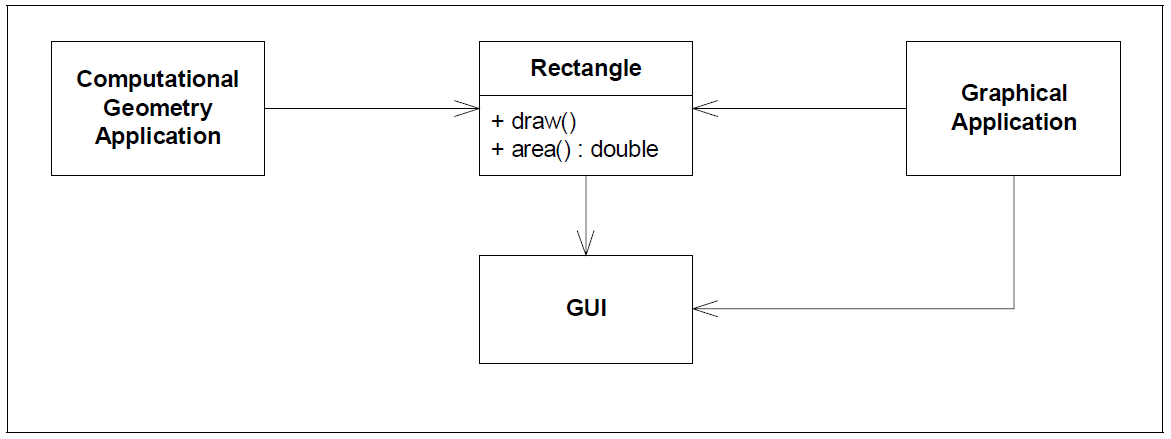
\includegraphics[width = \textwidth]{coupled_rectangle.PNG}
\end{figure}
\subsection{OCP}
Klasser, moduler, funktioner mm. Skal være åbne for udvidelser, men lukket for ændringer.

Der er sq ikke så meget til dette. Nøglen er abstraction. Hvis du laver to klasser som er direkte afhængige af hinanden, så overholder dette ikke ocp. Da disse ikke på nogen måde er åbne for udvidelser. Sørger du til gengæld at Klasse A er afhænging af interface IB som implementeres af B, så har du sørget for at du kan udvide IB med en ny implementering. 
Et andet eksempel handler om shapes. Hvis du har en funktion som skal tegne alle de shapes som du har og du har defineret funktionen til at tegne alle dem du selv har implementeret, så er den lukket for udvidelse. Hvis du derimod lavet et shape interface med funktionen draw, også senere lave en liste med disse shapes, så er det åben for at andre kan skrive shapes som opfylder dit shape interface, uden at skulle ændre metoden drawallshapes
\subsection{LSP}
Der er et godt meme som siger hvis ``if it looks like a duck, quacks like a duck, but need batteries - you probably have the wrong abstraction''
En afledt klasse må IKKE:
\begin{enumerate}
    \item remove base class behavior
    \item violate base class invariants
\end{enumerate}
\subsection{Interface Segregation Principle}

Du må ikke tvinge en bruger til at implementere et interface 
for kun 2/3 dele af det er nødvendigt

kort sagt så betyder det altså hvis du har et interface med f.eks 3 funktioner. Og disse 3 funktioner ikke nødvendigvis skal bruges i hver implementering af interfaces, så bryder du altså denne regl, og burde splitte dit interface op i 2.
\subsection{DIP}
INJEEECT
\end{document}